\subsection{Lentes y formación de imágenes}

Para empezar comencemos recordando que cuando un rayo de luz pasa de un medio con índice de refracción \(n_1\) a otro con índice \(n_2\), y atraviesa una superficie plana, la dirección del rayo cambia de acuerdo con la Ley de Snell:

\[
n_1 \sin \theta_1 = n_2 \sin \theta_2
\]

\subsubsection{Refacción en una superficie esférica}

Consideremos una única superficie esférica de radio \(R\), separando dos medios de índices \(n_1\) y \(n_2\). Un objeto colocado en el medio \(n_1\) yace frente a la superficie esférica en el punto \(O\). Los rayos que salen de \(O\) divergen y reflejan en la superficie esférica, formando un haz que converge en el punto \(I\). 

En la figura \ref{fig:lens_refraction} se muestra esta situación, pero solo se ha dibujado un rayo incidente y un rayo refractado para ilustrar la idea.
\begin{figure}[ht]
  \centering
  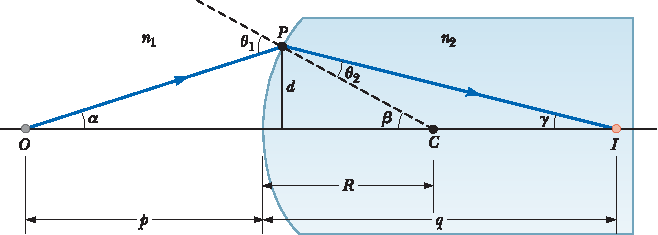
\includegraphics[width=\textwidth]{lens_refraction.pdf}
  \caption{Imagen formada por refracción en una superficie esférica.}
  \label{fig:lens_refraction}
\end{figure}

Para aproximaciones paraxiales\footnote{La aproximación paraxial se utiliza para el cálculo de sistemas ópticos, suponiendo que las trayectorias de los rayos de luz forman ángulos pequeños con el eje óptico.} (ángulos pequeños en radianes), se puede hacer \(\sin \theta \approx \tan \theta \approx \theta\), y se puede reescribir la ecuación de Snell como:
\[
  n_1 \theta_1 = n_2 \theta_2
\]

Se sabe que el ángulo externo de un triángulo es igual a la suma de los ángulos internos no adyacentes (ver demostración en la sección adicional: \ref{sec:suma_angulos_internos}). Así que:
\begin{align*}
  \theta_1 =& \alpha + \beta \\
  \beta =& \theta_2 + \gamma
\end{align*}
Si combina las tres expresiones y elimina \(\theta_1\) y \(\theta_2\), obtiene:
\begin{equation}
  n_1 \alpha + n_2 \gamma = (n_2 - n_1) \beta
\end{equation}

Y como estamos trabajando con aproximaciones paraxiales:
\begin{align*}
  \tan \alpha \approx &\alpha \approx \frac{d}{p} \\
  \tan \beta \approx &\beta \approx \frac{d}{R} \\
  \tan \gamma \approx &\gamma \approx \frac{d}{q}
\end{align*}
Podemos reescribir la expresión como sigue:
\begin{equation}
\frac{n_1}{p} + \frac{n_2}{q} = \frac{n_2 - n_1}{R}
\label{eq:refraction_spherical}
\end{equation}

Donde:
\begin{itemize}
  \item \(p\): distancia desde el objeto hasta la superficie (en el medio 1),
  \item \(q\): distancia desde la imagen hasta la superficie (en el medio 2),
  \item \(R\): radio de curvatura de la superficie (positivo si el centro de curvatura está del lado del medio 2),
  \item \(n_1\): índice de refracción del medio de entrada,
  \item \(n_2\): índice de refracción del medio de salida.
\end{itemize}

\begin{tcolorbox}[myconclusion]
  \textbf{Cuidado}: En los espejos, la luz se refleja y las imágenes reales (cuando ocurren) se forman del mismo lado que el objeto.
  En cambio, en la refracción (como con lentes), los rayos de luz se desvían y convergen al otro lado del medio, por lo que la imagen se forma detrás de la superficie refractante, no del mismo lado del objeto.
\end{tcolorbox}

\noindent Esto implica que los signos serán al revés que en los espejos, quedando la siguiente regla convencional de signos:
\begin{enumerate}
  \item El lado de la superficie en el cual se originan los rayos luminosos se define como \textit{cara frontal}. El otro lado se llama \textit{cara trasera}.
  \item Identifique la localización del objeto \(p\) teniendo en cuenta:
    \begin{itemize}
      \item el objeto está delante de la superficie: \textit{objeto real} (positivo)
      \item el objeto está detrás de la superficie: \textit{objeto virtual} (negativo)
    \end{itemize}
  \item  Localización de la imagen \(q\):
    \begin{itemize}
      \item la imagen está detrás de la superficie: \textit{imagen real} (positiva)
      \item la imagen está delante de la superficie: \textit{imagen virtual} (negativa)
    \end{itemize}
  \item Altura de la imagen \(h'\):
    \begin{itemize}
      \item la imagen no es invertida: \(h' > 0\) (positiva)
      \item la imagen es invertida: \(h' < 0\) (negativa)
    \end{itemize}
  \item Distancia focal \(f\) y radio \(R\):
    \begin{itemize}
      \item Es positiva cuando el centro de curvatura está del lado del medio 2
      \item Es negativa cuando el centro de curvatura está del lado del medio 1
    \end{itemize}
\end{enumerate}

\subsubsection{Refacción en una superficie plana}

\begin{wrapfigure}{r}{0.28\textwidth}
  \centering
  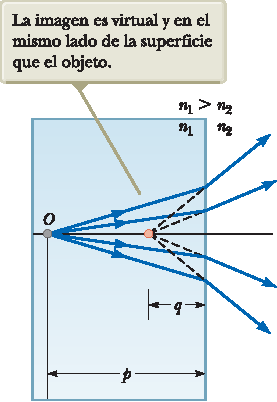
\includegraphics[width=\linewidth]{plane_surface_refraction.pdf}
  \caption{Refacción en una superficie plana.}
  \label{fig:plane_surface_refraction}
\end{wrapfigure}
Para una superficie plana, el eje óptico es perpendicular a la superficie. Tomando la ecuación \ref{eq:refraction_spherical} y suponiendo que el radio de curvatura es infinito, obtenemos la ecuación de refracción para una superficie plana:
\begin{align}
  \frac{n_1}{p} + \frac{n_2}{q} &= 0 \notag \\
  q &= -\frac{n_1}{n_2} p
\end{align}

\noindent donde:
\begin{itemize}
  \item \(p\) es la distancia del objeto a la superficie (en el medio 1),
  \item \(q\) es la distancia de la imagen a la superficie (en el medio 2),
  \item \(n_1\) y \(n_2\) son los índices de refracción.
\end{itemize}

De esta ecuación se puede ver que el signo de \(q\) es opuesto a \(p\), lo que implica que la imagen se forma en el otro lado del medio.

\subsection{Imágenes formadas por lentes delgadas}

Una lente delgada es una combinación de dos superficies esféricas, muy cercanas entre sí comparadas con las distancias del objeto y la imagen.
\begin{figure}[ht]
  \centering
  \begin{subfigure}[b]{0.45\textwidth}
      \centering
      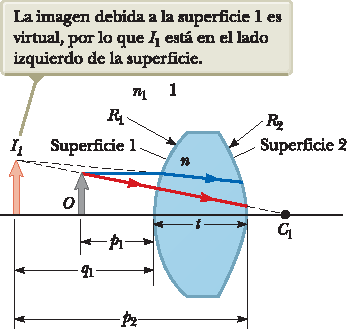
\includegraphics[width=\textwidth]{lens_a.pdf}
      \caption{Lente con imagen virtual.}
      \label{fig:lens_a}
  \end{subfigure}
  \hfill
  \begin{subfigure}[b]{0.45\textwidth}
      \centering
      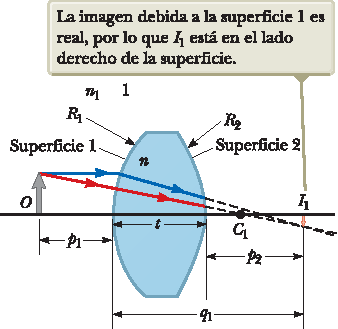
\includegraphics[width=\textwidth]{lens_b.pdf}
      \caption{Lente con imagen real.}
      \label{fig:lens_b}
  \end{subfigure}
  \caption{Para localizar la imagen formada por una lente, utilice la imagen virtual en \(I_1\) formada por la superficie \(1\) como el objeto para la imagen formada por la superficie \(2\). El punto \(C_1\) es el centro de la curvatura de la superficie \(1\).}
  \label{fig:lenses}
\end{figure}

Supongamos una lente delgada en el aire (\(n_{\text{aire}} = 1\)), hecha de un material con índice de refracción \(n\). Las dos superficies tienen radios \(R_1\) y \(R_2\). Luego se coloca un objeto en el punto \(O\) a una distancia \(p_1\) enfrente de la superficie \(1\).

Se aplica la fórmula de la superficie esférica (ecuación \ref{eq:refraction_spherical}) dos veces: una para cada cara de la lente.

\textbf{Primera refracción} (cara con radio \(R_1\) - figura \ref{fig:lens_a}):

\[
\frac{1}{p_1} + \frac{n}{q_1} = \frac{n - 1}{R_1}
\]
donde \(q_1\) es la posición de la imagen debida a la superficie \(1\). Si la imagen es virtual, \(q_1\) será negativa, sino será positiva.

\textbf{Segunda refracción} (cara con radio \(R_2\) - figura \ref{fig:lens_b}):

\noindent Para la superficie \(2\) se tiene \(n_1 = n\) y \(n_2 = 1\). Si \(p_2\) es la distancia objeto de la superficie \(2\) y \(q_2\) es la distancia a la imagen:

\[
\frac{n}{p_2} + \frac{1}{q_2} = \frac{1 - n}{R_2}
\]
Ahora hay que introducir, en términos matemáticos, el hecho de que la \hl{imagen} formada por la primera superficie actúa como el objeto para la segunda superficie. Podemos ver en la figuras \ref{fig:lens_a} (caso de imagen virtual, \(q_1 < 0\)) y \ref{fig:lens_b} (caso de imagen real, \(q_1 > 0\)) que \(p_2 = -q_1 + t\), donde \(t\) es el espesor del lente.

Si despreciamos el espesor del lente, obtenemos la ecuación de la lente delgada, siendo \(p_2 = -q_1\) se obtiene:
\[
  -\frac{n}{q_1} + \frac{1}{q_2} = \frac{1 - n}{R_2}
\]
Sumando ambas ecuaciones (primera refracción y segunda refracción):
\[
\frac{1}{p_1} + \frac{1}{q_2} = (n - 1)\left( \frac{1}{R_1} - \frac{1}{R_2} \right)
\]
como la lente es delgada, entonces se pueden eliminar los subíndices de \(p_1\) y \(q_2\), obteniendo:
\[
\frac{1}{p} + \frac{1}{q} = \frac{1}{f} = (n - 1)\left( \frac{1}{R_1} - \frac{1}{R_2} \right)
\]

Esta es la fórmula de lentes delgadas. Esta ecuación se conoce como \textbf{ecuación de los fabricantes de lentes} porque se utiliza para determinar los valores de \(R_1\) y \(R_2\) necesarios para un índice de refracción \(n\) dado y una distancia focal \(f\) deseada.

\subsection{Ecuación de la lente delgada en forma de distancia focal}

Definimos la distancia focal \(f\) como la posición donde se forma la imagen de un objeto en el infinito:

\[
\frac{1}{f} = (n - 1)\left( \frac{1}{R_1} - \frac{1}{R_2} \right)
\]

Entonces, la ecuación de la lente queda:

\[
\frac{1}{p_1} + \frac{1}{q} = \frac{1}{f}
\]
